\section{Tuesday, August 30th}
\subsection{Review: LTI Systems}

\begin{itemize}
    \item Signals are functions
    \begin{align*}
    &\text{Continuous Time: } x : \mathbb{R} \rightarrow \mathbb{R} 
    \text{ or } x : \mathbb{R} \rightarrow\mathbb{C}
    \\
    &\text{Discrete Time: } x :  \mathbb{Z} \rightarrow \mathbb{R} \text{ or } \mathbb{C}
    \end{align*}
    \[
        X \quad\quad Y
    \]
    \[
        x \ \texttt{->} \ \boxed{H} \ \texttt{->} \  y
    \]
    where $X$ is the input signal space and\\
    $Y$ is the output signal space.
    
    Formally, we can say that $y=H(x)$. Note that systems are just mappings from functions to functions.
    
    \begin{shaded}
    Time Invariance:\\
    If $\hat x(t)\stackrel{.} = x(t-T)$ then $\hat y(t) \stackrel.= y(t-T)$ must be offset but the same relative amount.
    \end{shaded}
    
    Easy way to check for LTI: ZIZO.\\
    To make sure that linearity is ensured, zero should map to zero. Note that this alone is not enough to prove linearity but it is necessary (ex. $y(t)=x^2(t)$).

    DT-LTI:    
    \[
        \delta(n) \ \texttt{->} \ \boxed{H} \ \texttt{->} \  h(n)
    \]
    
    Time-Invariance:
    \[
        \delta(n-k) \ \texttt{->} \ \boxed{H} \ \texttt{->} \  h(n-k)
    \]
    
    Scaling Property:
    \[
        x(k)\delta(n-k) \ \texttt{->} \ \boxed{H} \ \texttt{->} \  x(k)h(n-k)
    \]
    
    Additivity:
    \[
        x(n)=\sum_{k=-\infty}^\infty x(k)\delta(n-k) \ \texttt{->} \ \boxed{H} \ \texttt{->} \  \sum_{k=-\infty}^\infty x(k)h(n-k)
    \]
    
    The importance of LTI is that you get what is essentially invertibility, which can uniquely describe a signal by its impulse response. Note that LTI systems can be seen as Convolutions.
    
    \textbf{Convolution is commutative:}
    \[
        y(n) = (x\star h)(n)=\sum_{k=-\infty}^\infty x(k)h(n-k)
        = (h\star x)(n)
    \]
    
    Impulse Response of Cascade (Series) Interconnection:
    \[
        x(n)=\delta(n) \ \texttt{->} \ \boxed{f(n)} \ \texttt{->} \ \boxed{g(n)} \ \texttt{->} \  y(n)=(f\star g)(n)
    \]
    % Expect Parallel Interconnection in future lecture xor future exam
\end{itemize}


\subsection{Simple Moving Average}
\[
    x(n) \ \texttt{->} \ \boxed{h(n)} \ \texttt{->} \  y(n)=\frac1N\sum_{k=0}^{N-1} x(n-k)=\frac{x(n)+\cdots+x(n-N+1)}{N}
\]

\begin{enumerate}[label=(\alph*)]
    \item Determine $h(n)$ and Plot it.
    \begin{itemize}
        \item Let $x(n)=\delta(n),$ then $y(n)=h(n)=\frac{\delta(n)+\delta(n-1)+\cdots+\delta(n-(N-1))}{N}$
    
        \begin{figure}[h]
            \centering
            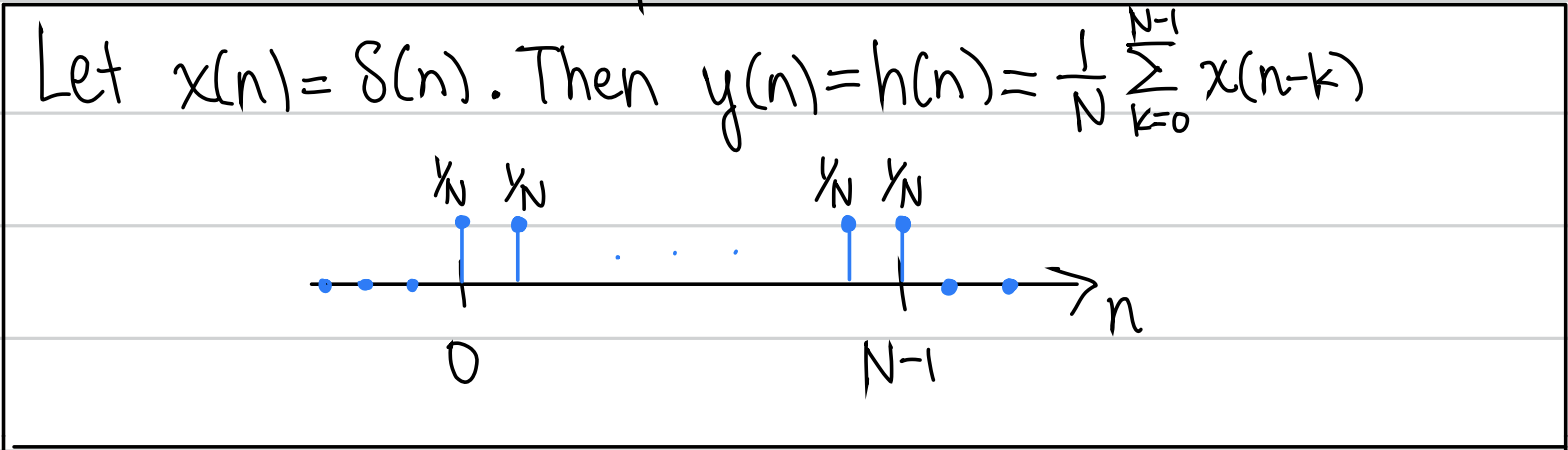
\includegraphics[scale=0.25]{lectures/img/Lec2_SimpleMovingAverage.png}
            \caption{Special thanks to Jonathan Pei for this drawing}
            \label{fig:simple_moving_average}
        \end{figure}
    \end{itemize}
\end{enumerate}

\subsection{Exponentially-Weighted Moving Average Filter}
Next time :)
